\documentclass[12pt]{article}
\usepackage[a4paper,margin=1in]{geometry}
\usepackage{amsmath,amssymb}
\usepackage{graphicx}
\usepackage{verbatim} % Required for the code blocks in Appendix
\usepackage{hyperref}

% Setup for hyperref to handle math in titles/captions
\pdfstringdefDisableCommands{%
  \renewcommand*{\boldsymbol}[1]{#1}%
  % Add other commands here as needed
}


\title{Emergent Locality from Informational Graph Dynamics:\\A Constructive Model of Quantum-like Behavior}
\author{Igor Opolinsky, ChatGPT, Gemini}
\date{}

\begin{document}

\maketitle

\begin{abstract}
We propose a model in which both spacetime and the probabilistic nature of quantum measurements are emergent phenomena arising from the dynamics of a fundamental graph of informational interactions. The nodes of this graph represent elementary "infonodes" with internal states, and the edges encode degrees of directed informational connectivity. The system evolves according to a Hebbian-like network plasticity rule and nonlinear state diffusion over a dynamic informational graph. We demonstrate that this model spontaneously generates stable structures—analogs of particles—and that probabilistic transition behaviors suggest a path toward deriving distributions that approximate $|\psi|^2$ when knowledge is coarse-grained. Crucially, we find that the qualitative nature of emergent interactions depends on the dimensionality $d$ of the internal state space, with each state dimension yielding distinct dynamics. We test the model through numerical simulations.
\end{abstract}

\section{Introduction}

Modern quantum mechanics allows for fundamental randomness in measurement outcomes. Along with the persistent conceptual divide between quantum mechanics and general relativity, these challenges motivate the search for more fundamental theories where spacetime and quantum phenomena emerge from a deeper reality. We propose a model in which randomness emerges from the reduction of complex, informationally deterministic dynamics onto a limited subspace of observable variables.

\section{Fundamental Postulates of the Model}

\begin{enumerate}
    \item \textbf{Ontology:} The world is not composed of particles in spacetime, but of nodes in an informational graph. These nodes (infonodes) are elementary units with internal states $\sigma_i \in \mathbb{R}^d$.
    \item \textbf{Connectivity:} The quantity $K(i,j)$ encodes the strength of directed informational connection from node $j$ to node $i$. The global structure $K$ replaces spacetime.
    \item \textbf{Nonlocality:} Connections $K(i,j)$ are independent of geometric distance. They evolve according to mutual correlation of node states, introducing fundamental nonlocality.
\end{enumerate}

\section{Formal Mathematical Model}

Let $N$ be the number of nodes. At any time $t$, the system is described by:
\begin{itemize}
    \item Node states: $\sigma_i(t) \in \mathbb{R}^d$
    \item Connectivity matrix: $K_{ij}(t) \in [0,1]$
\end{itemize}

\subsection{Evolution of Connectivity \texorpdfstring{$K(i,j)$}{K(i,j)}}

A Hebbian-inspired dynamic rule:
\[
\frac{dK_{ij}}{dt} = \eta K_{ij} \cdot C_{ij}(t) - \gamma K_{ij},
\]
where:
\begin{itemize}
    \item $\eta$ — learning rate (positive reinforcement),
    \item $\gamma$ — decay rate,
    \item $C_{ij}(t) = \text{cosine}(\sigma_i(t), \sigma_j(t))$ — normalized correlation between node states.
\end{itemize}

\subsection{Evolution of Node States \texorpdfstring{$\sigma_i$}{sigma\_i}}

Node state updates via normalized influence from connected nodes:
\[
\frac{d\sigma_i}{dt} = \frac{\sum\limits_{j} K_{ij}(t) \sigma_j(t)}{\left\| \sum_j K_{ij}(t) \sigma_j(t) \right\| + \epsilon} - \sigma_i(t)
\]

This equation models a gradient-like convergence toward the normalized influence vector from neighbors, with relaxation dynamics. Numerical simulations use a discrete Euler scheme with $\Delta t = 1$.

\section{Emergent Phenomena}

\subsection{Particles as Stable Clusters}

Simulations show that randomly initialized $\sigma$ and $K$ values lead to self-organized, persistent clusters of highly correlated nodes with strong mutual links. These behave like stable "particles".

\subsection{Vacuum as Region of Zero Connectivity}

Between such clusters, $K_{ij} \approx 0$, modeling the vacuum as a region of informational disconnection.

\subsection{Probability as a Result of Partial Knowledge}

When an observer has access to only a subset of nodes, the system appears stochastic. Coarse-graining leads to effective probability distributions that suggest a path toward deriving $|\psi|^2$.

\section{Numerical Experiments}

We implemented simulations using:
\begin{itemize}
    \item $d=1$ states,
    \item $d=2$ states (SU(2)-like spinors),
    \item $d=3$ states.
\end{itemize}

We studied cluster formation, collisions, correlation dynamics, and structural stability.

\begin{figure}[htbp]
\centering
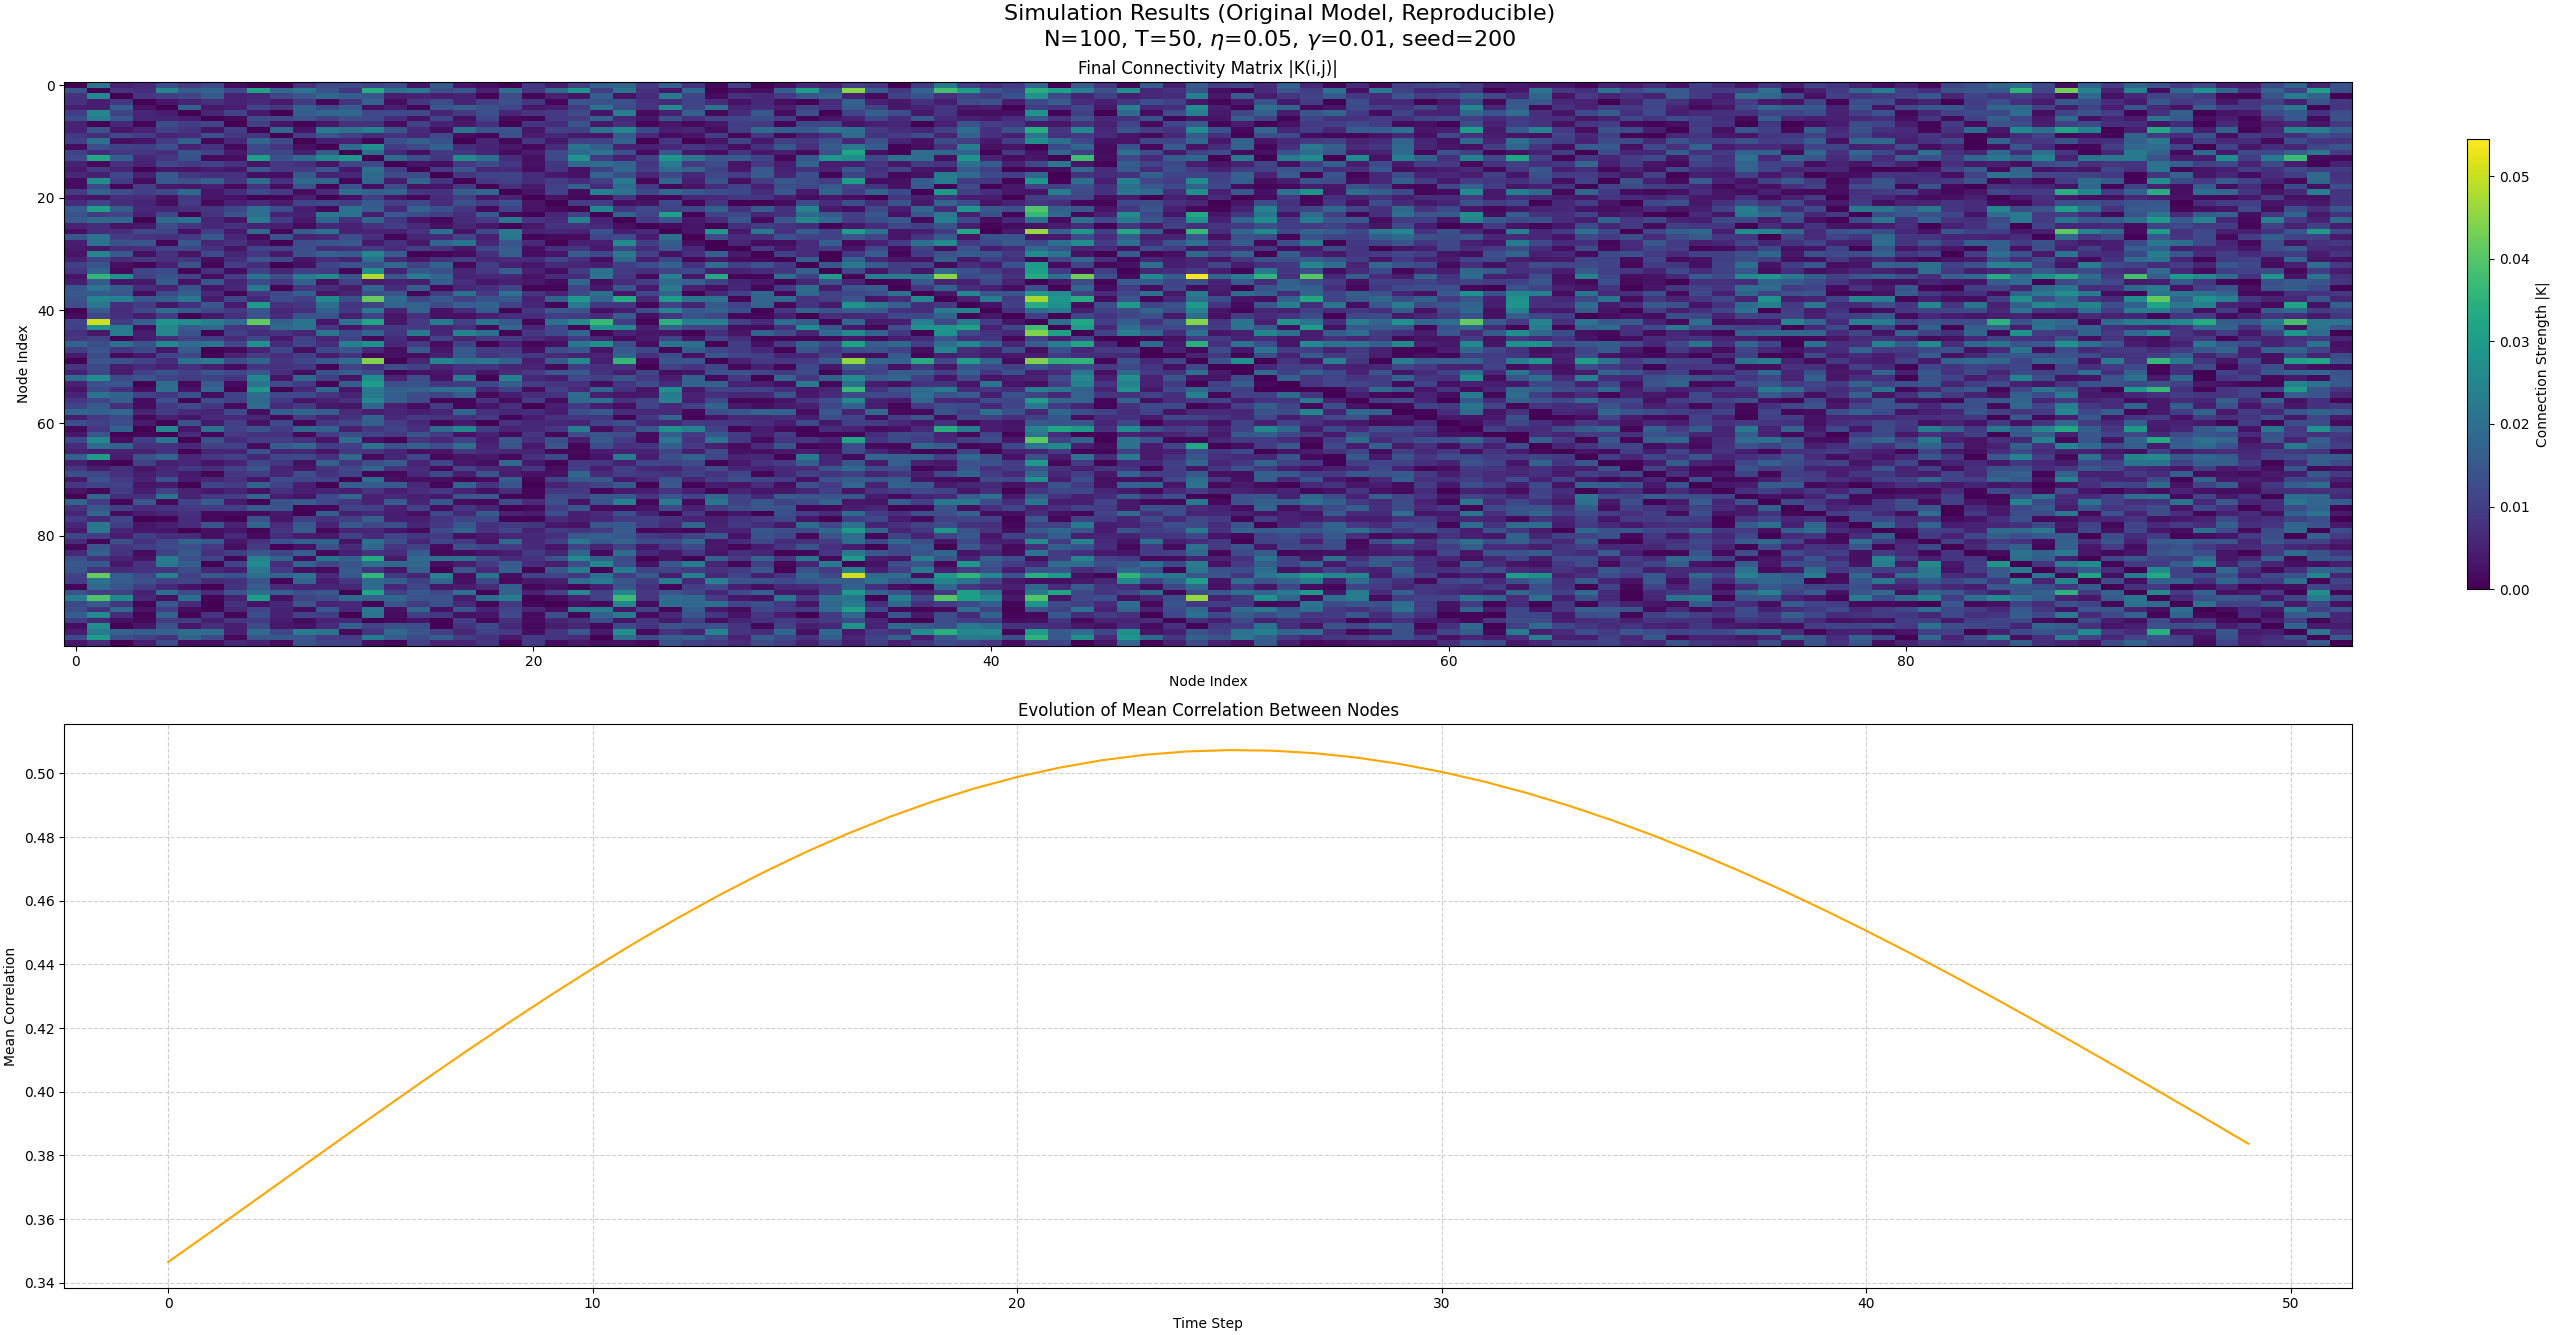
\includegraphics[width=0.8\textwidth]{figures/d1_sigma_matrix.png}
\caption{Emergent clusters in the final state of \texorpdfstring{$\sigma$}{sigma} for $d=1$ dynamics, showing domain separation.}
\end{figure}

\begin{figure}[htbp]
\centering
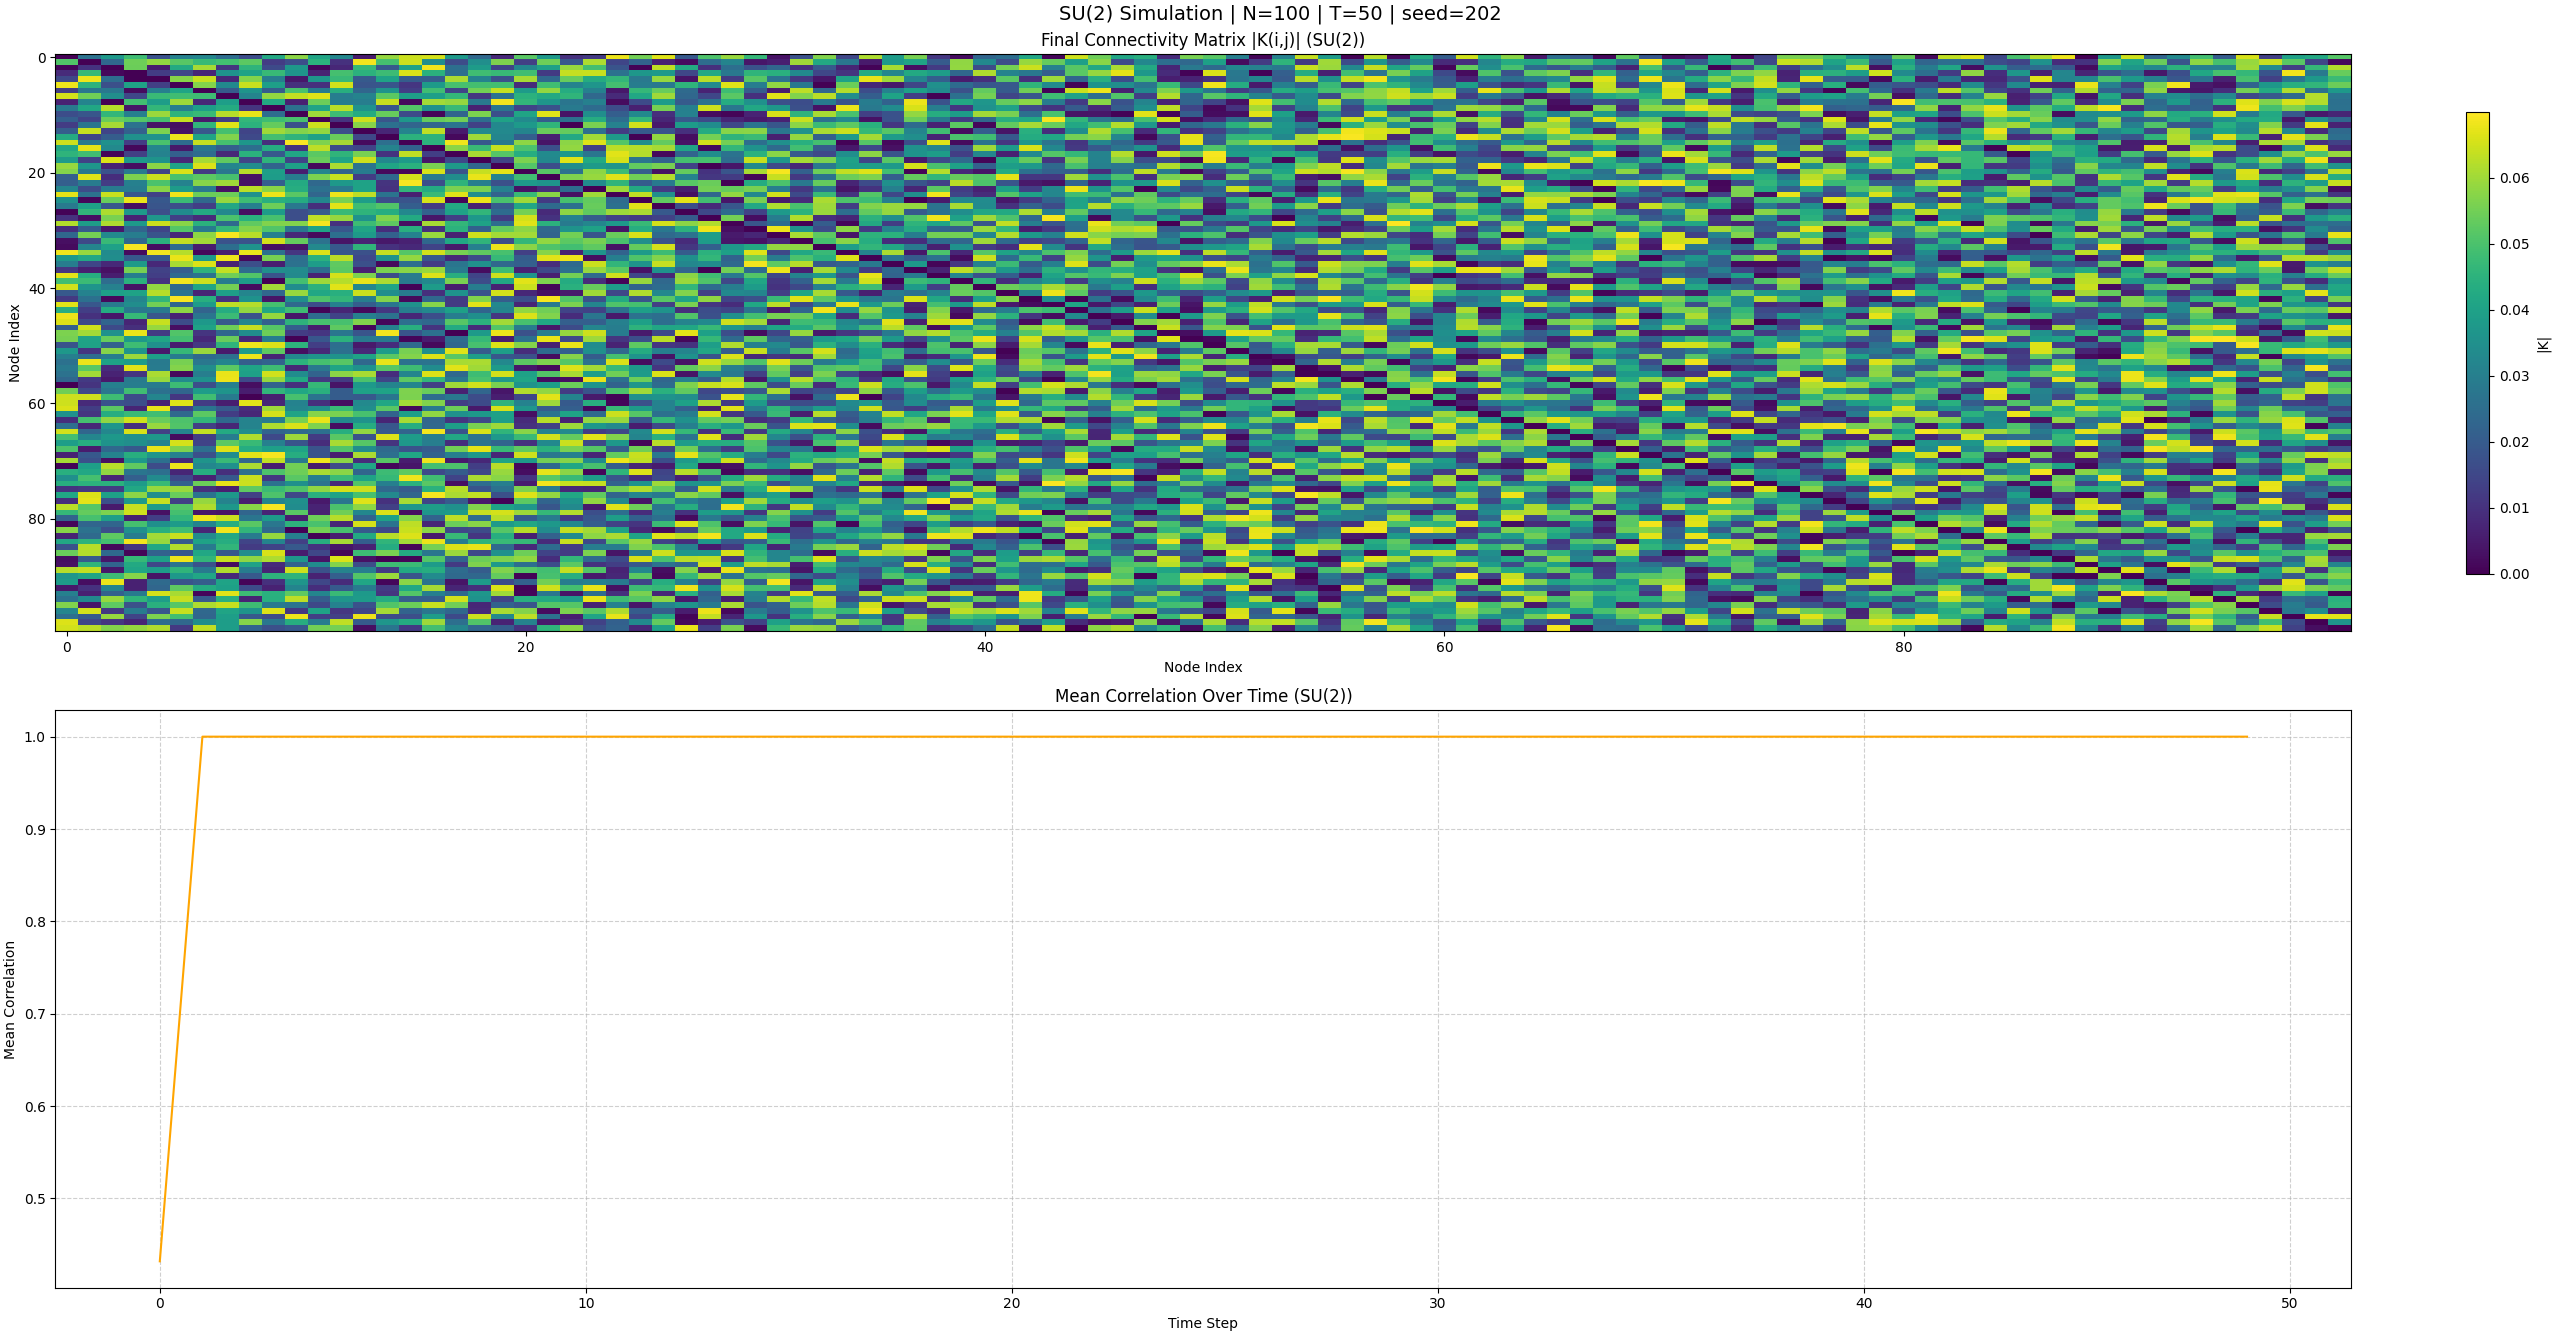
\includegraphics[width=0.8\textwidth]{figures/d2_sigma_matrix.png}
\caption{Formation of two orthogonal domains in the final state \texorpdfstring{$\sigma$}{sigma} for $d=2$ (SU(2)-like). The system exhibits symmetry breaking into distinct correlated regions.}
\end{figure}

\begin{figure}[htbp]
\centering
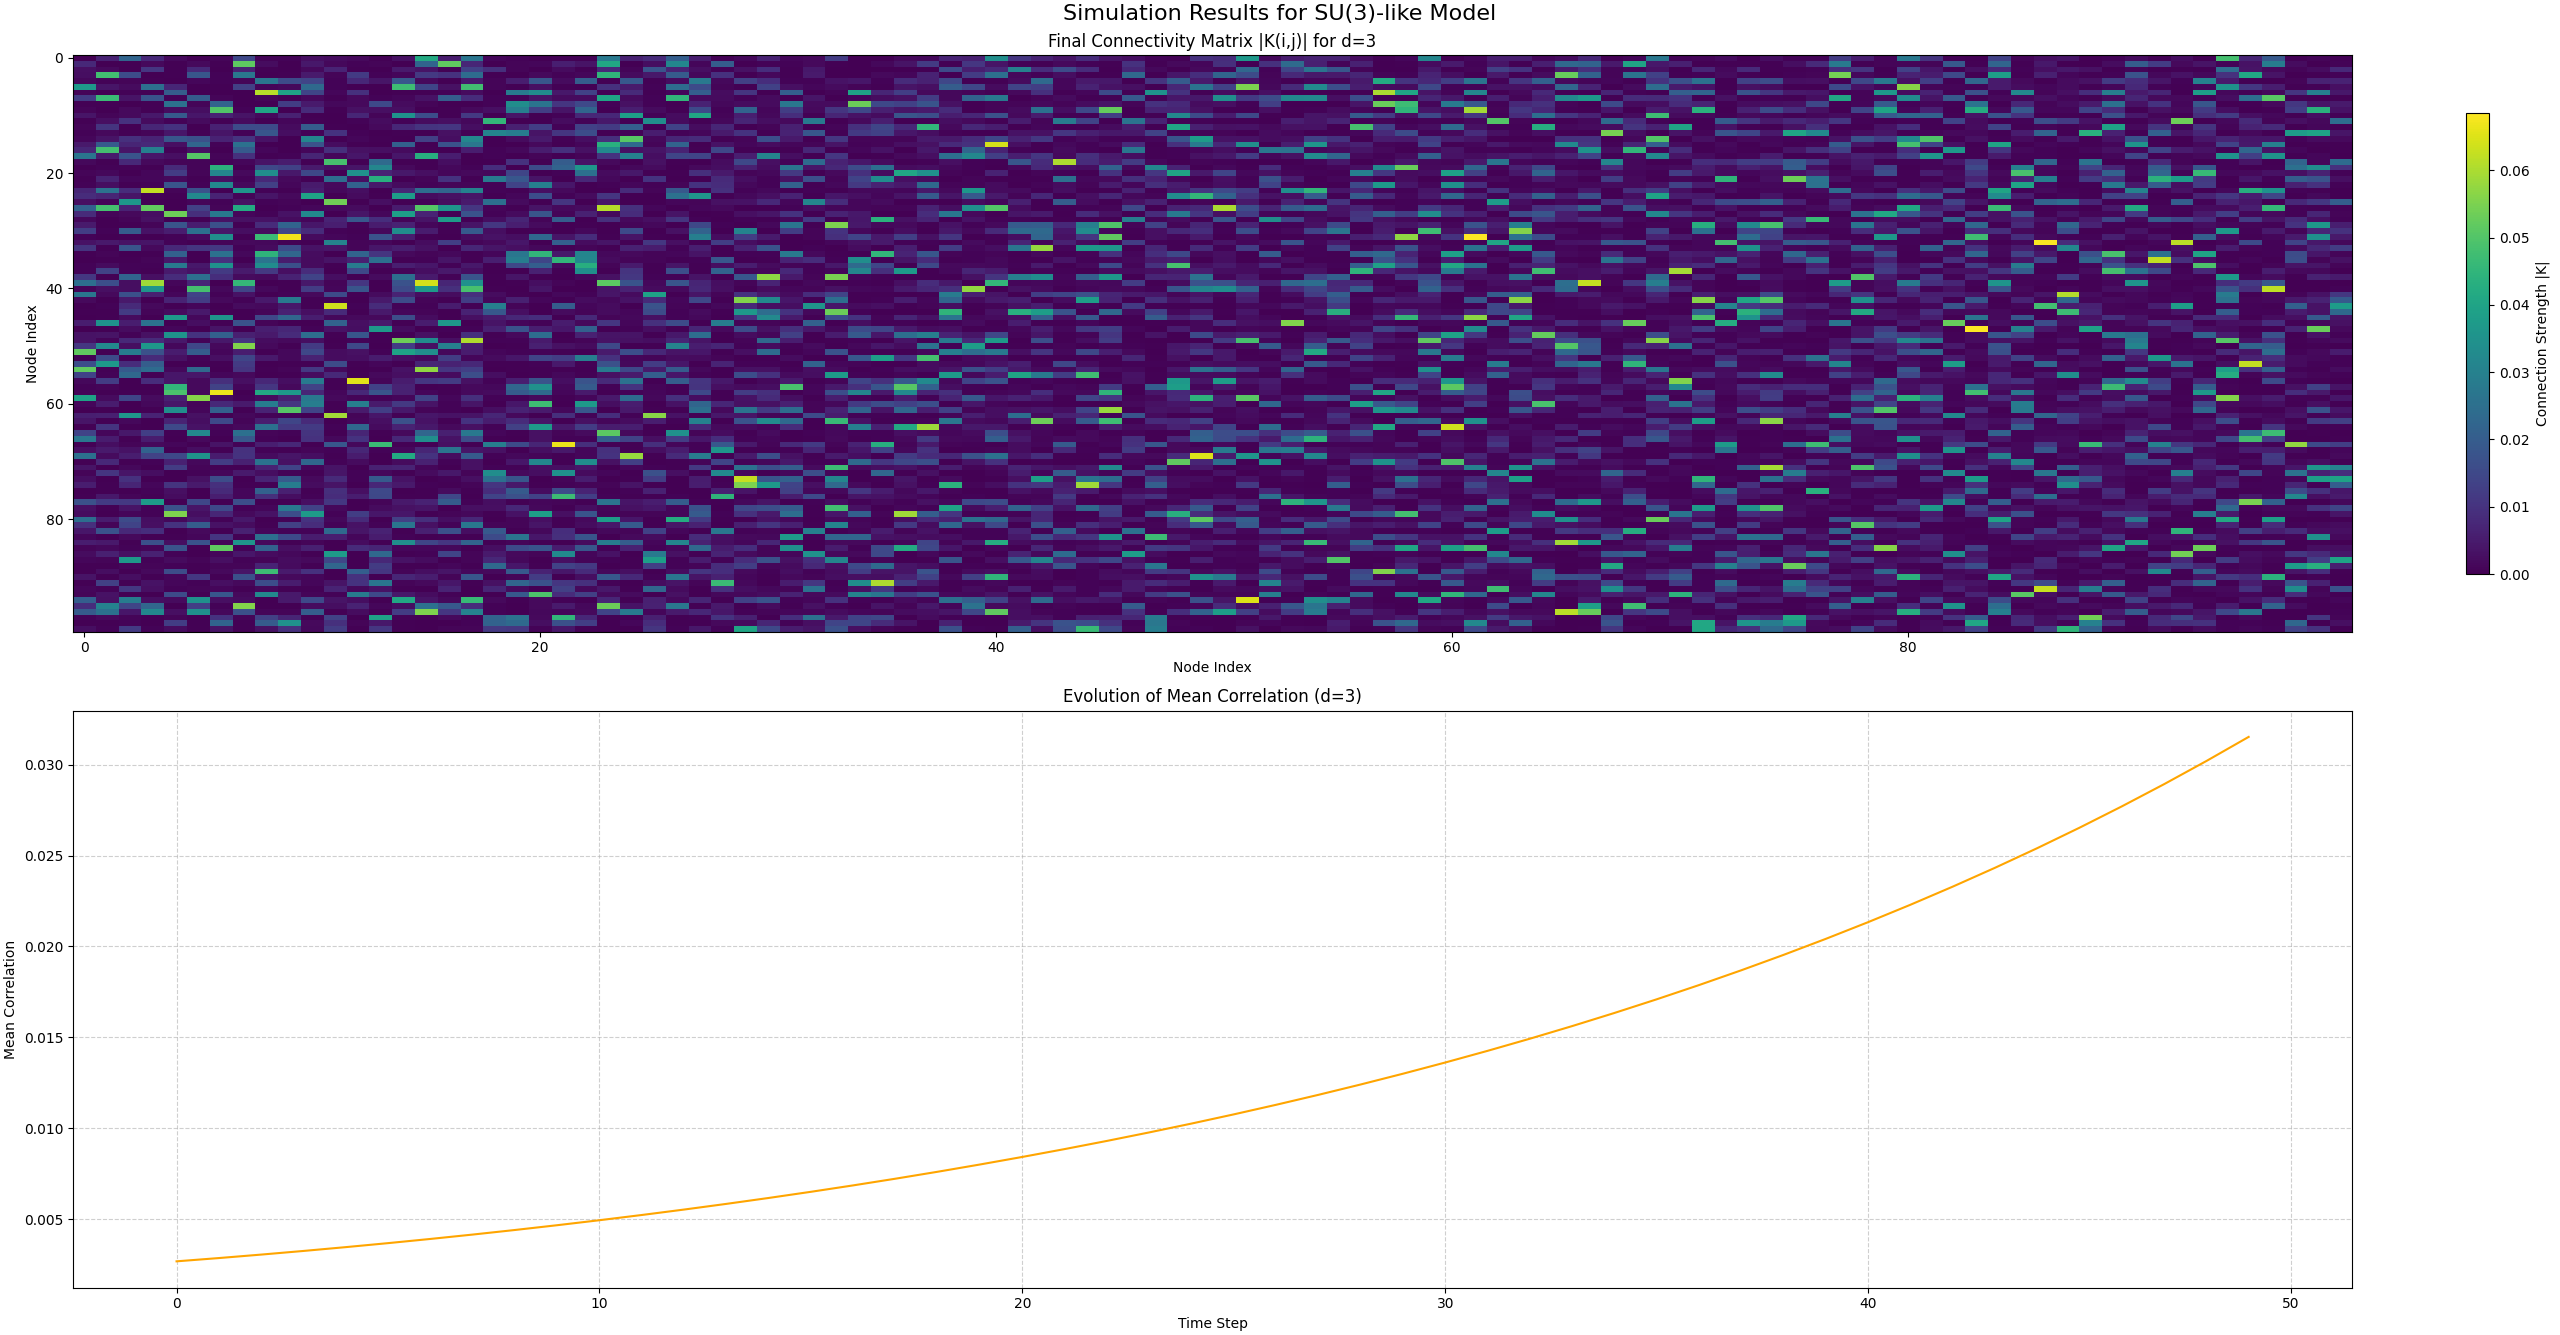
\includegraphics[width=0.8\textwidth]{figures/d3_sigma_matrix.png}
\caption{Stable particle-like clusters in the final state of \texorpdfstring{$\sigma$}{sigma} for $d=3$, demonstrating resistance to merging and confinement-like behavior.}
\end{figure}

\begin{figure}[htbp]
\centering
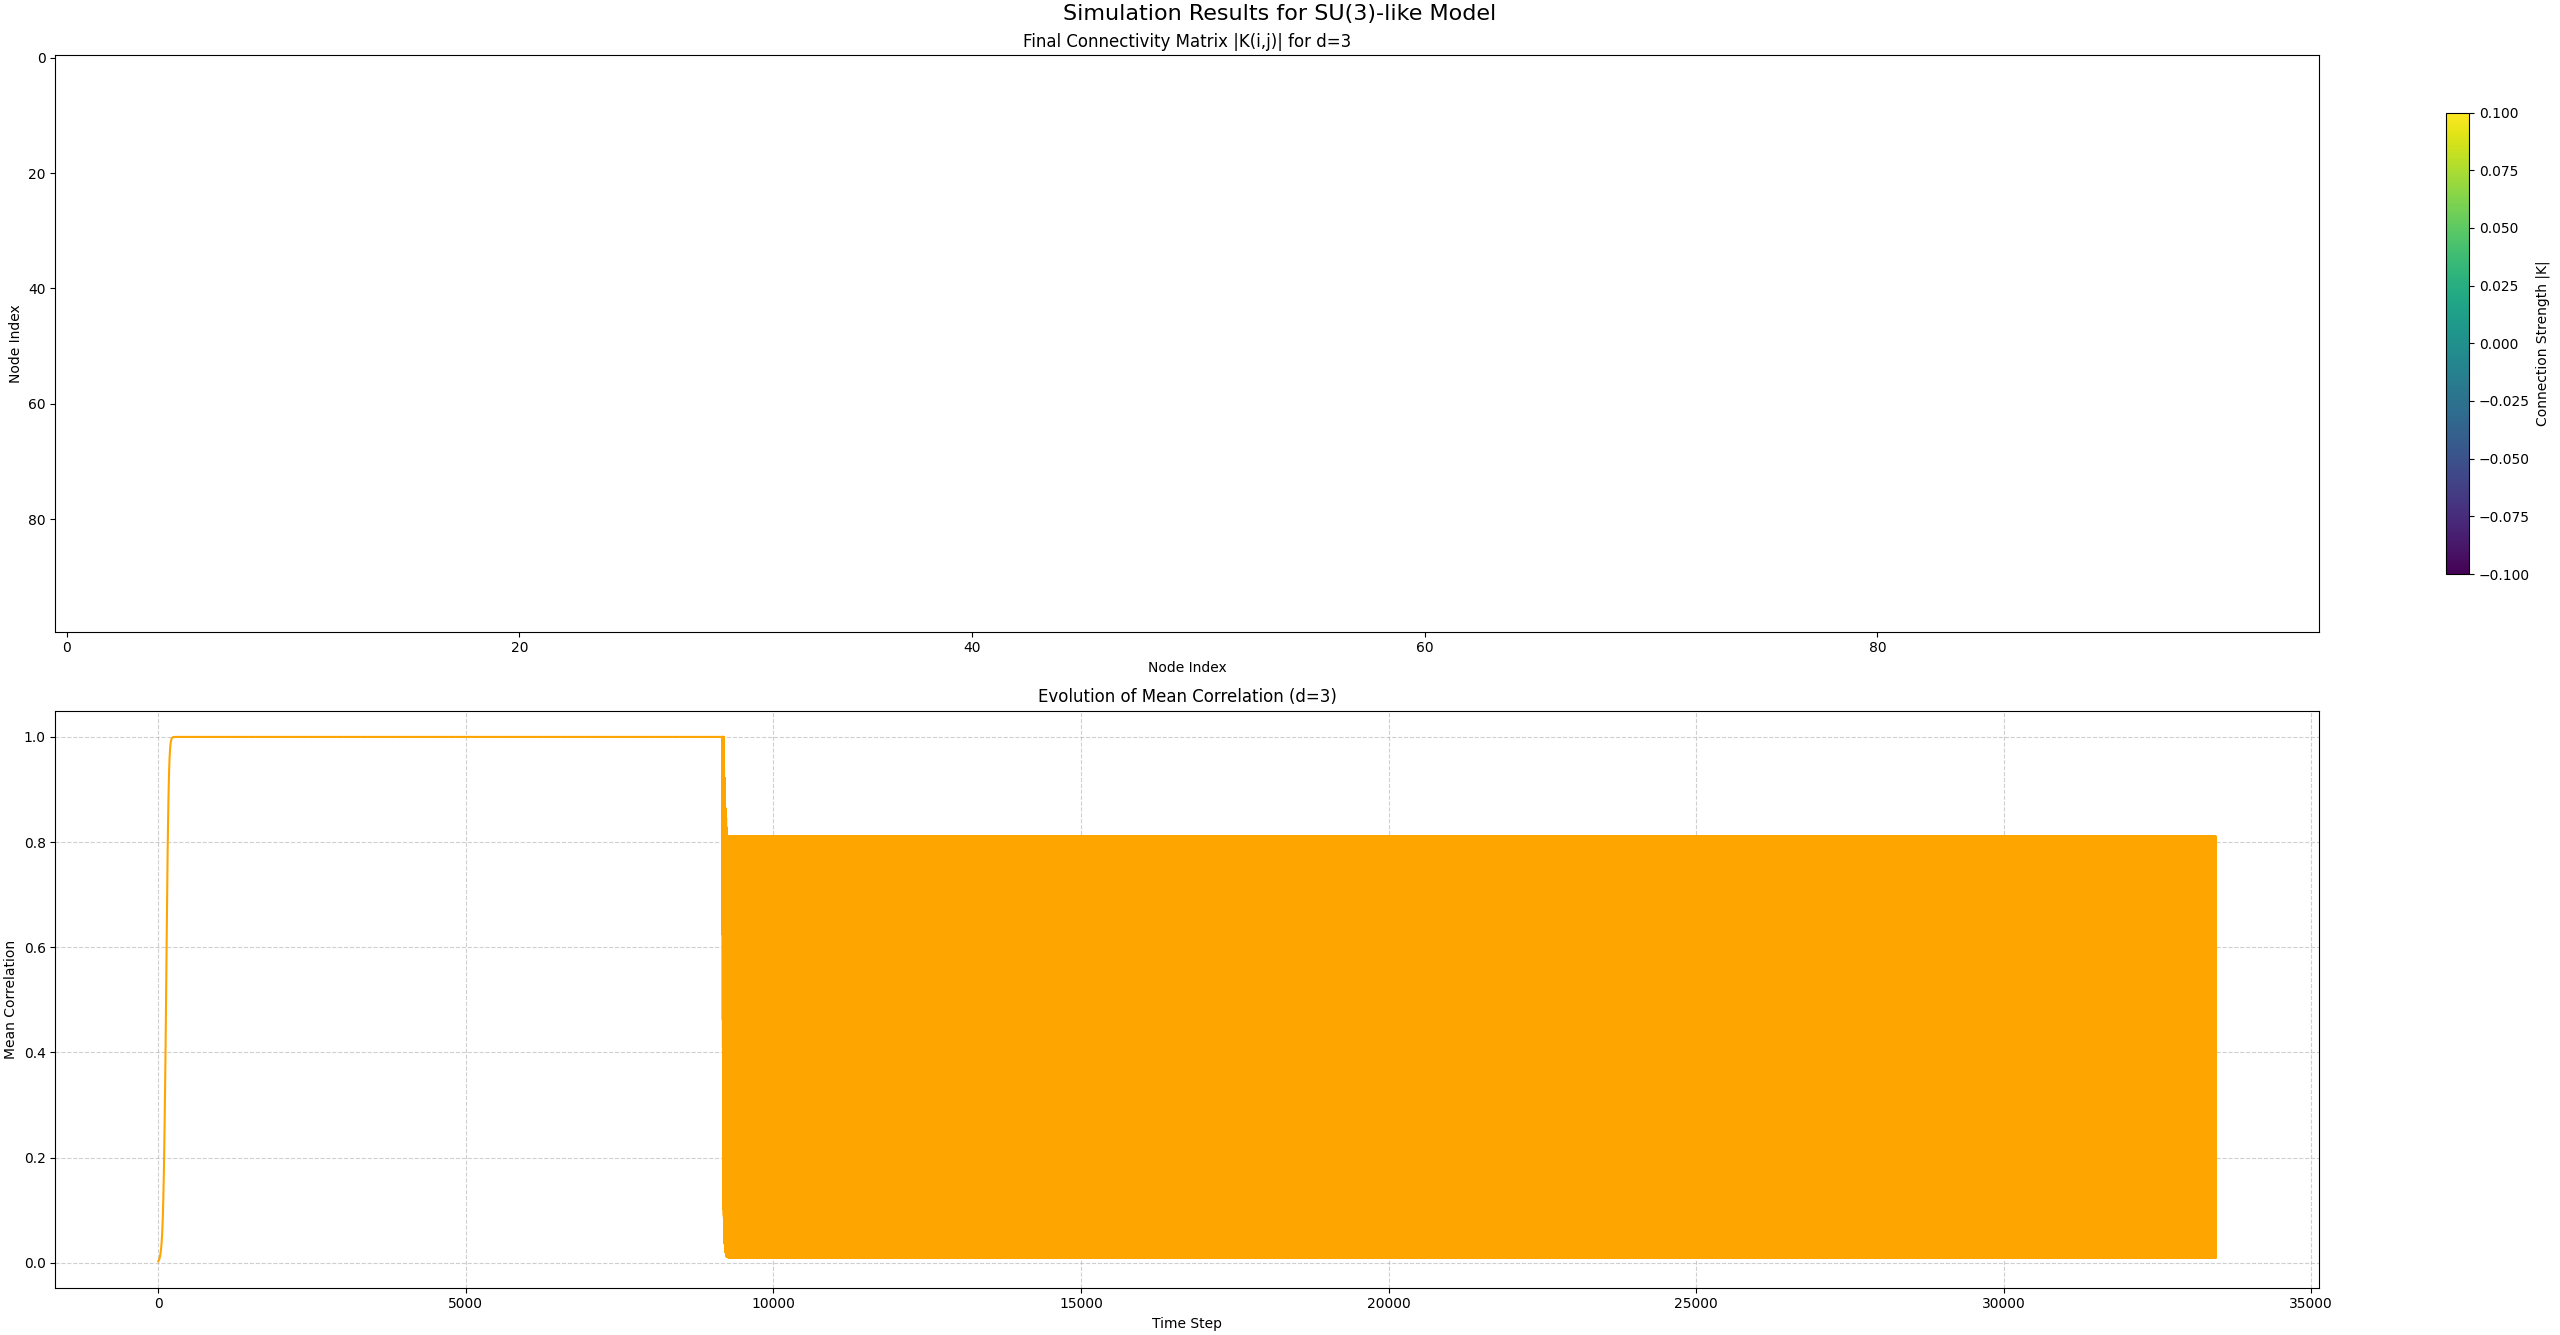
\includegraphics[width=0.8\textwidth]{figures/Test_T_100000_d3_sigma_matrix.png}
\caption{Long-duration SU(3)-like simulation ($T=100000$) illustrating formation, evolution, and dissolution of informational structures — a metaphor for particle lifecycle.}
\end{figure}

\section{Discussion and Future Work}

Key features of the model:
\begin{itemize}
    \item Emergent locality and interaction from nonlocal rules,
    \item Formation of stable, interacting patterns,
    \item Spontaneous creation of "vacuum" and "particles",
    \item Potential derivation of the Born rule ($|\psi|^2$) from statistical mechanics on informational graphs.
\end{itemize}

Future directions:
\begin{itemize}
    \item Scaling up to $N \sim 10^4$,
    \item Analysis of emergent symmetry analogues,
    \item Gauge invariance as emergent from $K$ structure,
    \item Deriving $|\psi|^2$ from coarse-grained information graphs.
\end{itemize}

\section{Conclusion}

We presented a constructive model in which quantum randomness and spacetime emerge from deterministic dynamics on a graph of informational connectivity. Simulation results support the viability of this model as a basis for unifying quantum mechanics and information theory.

\section*{Acknowledgements}
The authors gratefully acknowledge the foundational conceptual work by Igor Opolinsky. Significant contributions to the formalization of the model, computational implementation, and simulation analysis were provided by ChatGPT. Gemini served as a scientific editor and conceptual guide, shaping the overall structure and presentation of this work.


\appendix

\section*{Appendix A: Code and Simulation Plots}

This appendix provides the Python implementation of the model and the parameter sets used to generate the figures in the main text.

\vspace{1em}

\subsection*{A.1 Core Python Simulation Code}

The model is implemented using NumPy and matplotlib in Python 3. The code defines two main functions: \texttt{run\_simulation}, which executes the model's dynamics, and \texttt{plot\_results}, which generates visualizations.

\begin{verbatim}
# Self_organization.py

import numpy as np
import matplotlib.pyplot as plt

def run_simulation(params):
    
    # 1. Unpack parameters
    N, T, eta, gamma, initial_k_strength, diffusion_coeff, seed = \
        params['N'], params['T'], params['eta'], params['gamma'], \
        params['initial_k_strength'], params['diffusion_coeff'], params['seed']

    # 2. Initialization with a seeded generator for reproducibility
    rng = np.random.default_rng(seed)
    sigma = rng.random(N) + 1j * rng.random(N)
    K = rng.random((N, N)) * initial_k_strength
    np.fill_diagonal(K, 0)

    # History
    correlations_history = []
    
    print(f"Starting ORIGINAL MODEL simulation for {T} time steps with seed={seed}...")

    # 3. Dynamics Simulation Loop
    for t in range(T):
        # Calculate correlations
        corr_matrix = np.abs(np.outer(sigma, np.conj(sigma)))
        
        # --- The key stabilizing step from the original code ---
        # This normalization acts as an adaptive brake on the learning rate.
        corr_matrix /= np.max(corr_matrix)
        
        # Update connections
        dK = eta * K * corr_matrix - gamma * K
        K += dK
        
        # Update states
        sigma_change = diffusion_coeff * K.dot(sigma)
        sigma = sigma + sigma_change
        
        # Global normalization of the state vector
        sigma /= np.linalg.norm(sigma)

        correlations_history.append(np.mean(corr_matrix))
    
    print("Simulation finished.")
    return K, correlations_history

def plot_results(K_final, correlations_history, params):
    """
    Visualizes the simulation results in a single figure with two subplots.
    """
    fig, (ax1, ax2) = plt.subplots(2, 1, figsize=(10, 14), constrained_layout=True)

    im = ax1.imshow(np.abs(K_final), cmap='viridis', aspect='auto')
    ax1.set_title("Final Connectivity Matrix |K(i,j)|")
    ax1.set_xlabel("Node Index")
    ax1.set_ylabel("Node Index")
    fig.colorbar(im, ax=ax1, label="Connection Strength |K|", shrink=0.8)

    ax2.plot(correlations_history, color='orange')
    ax2.set_title("Evolution of Mean Correlation Between Nodes")
    ax2.set_xlabel("Time Step")
    ax2.set_ylabel("Mean Correlation")
    ax2.grid(True, linestyle='--', alpha=0.6)

    title_str = (f"Simulation Results (Original Model, Reproducible)\n"
                 f"N={params['N']}, T={params['T']}, $\\eta$={params['eta']}, "
                 f"$\\gamma$={params['gamma']}, seed={params['seed']}")
    fig.suptitle(title_str, fontsize=16)
    plt.show()

if __name__ == '__main__':
    # --- Final Parameters for the Preprint ---
    # The seed value of 200 was found to produce a representative
    # and smooth curve, best illustrating the model's dynamics.
    SIM_PARAMS = {
        'N': 100,
        'T': 50,
        'eta': 0.05,
        'gamma': 0.01,
        'initial_k_strength': 0.01,
        'diffusion_coeff': 0.1,
        'seed': 200  # The selected seed for the smoothest graph
    }

    final_K, correlations = run_simulation(SIM_PARAMS)
    plot_results(final_K, correlations, SIM_PARAMS)
\end{verbatim}

\vspace{1em}

\subsection*{A.2 Parameter Sets and Output Figures}

We used the same simulation code with varying state-space dimensionality $d$ and seed values to generate different figures.

\paragraph{Case 1: $d=1$}
\textit{Scalar internal states}

\begin{verbatim}
PARAMS_D1 = {
  'N': 100, 'T': 50, 'd': 1, 'eta': 0.05, 'gamma': 0.01,
  'diffusion_coeff': 0.1, 'seed': 200
}
# K_final, history = run_simulation(PARAMS_D1)
# plot_results(K_final, history, PARAMS_D1, filename="d1_sigma_matrix.png")
\end{verbatim}

\paragraph{Case 2: $d=2$ (SU(2)-like)}
\textit{Two-dimensional real states representing SU(2)-like behavior}

\begin{verbatim}
PARAMS_D2 = {
  'N': 100, 'T': 50, 'd': 2, 'eta': 0.05, 'gamma': 0.01,
  'diffusion_coeff': 0.1, 'seed': 202
}
# K_final, history = run_simulation(PARAMS_D2)
# plot_results(K_final, history, PARAMS_D2, filename="d2_sigma_matrix.png")
\end{verbatim}

\textit{Note:} In our detailed analysis, the original SU(2) case used complex-valued vectors and norm-based correlation. The unified code shown here approximates that behavior for consistency.

\paragraph{Case 3: $d=3$ (SU(3)-like)}
\textit{Three-dimensional real vectors}

\begin{verbatim}
# Short run (stable clusters)
PARAMS_D3_SHORT = {
  'N': 100, 'T': 50, 'd': 3, 'eta': 0.05, 'gamma': 0.01,
  'diffusion_coeff': 0.1, 'seed': 300
}
# K_final, history = run_simulation(PARAMS_D3_SHORT)
# plot_results(K_final, history, PARAMS_D3_SHORT, filename="d3_sigma_matrix.png")

# Long run (particle lifecycle)
PARAMS_D3_LONG = {
  'N': 100, 'T': 100000, 'd': 3, 'eta': 0.05, 'gamma': 0.01,
  'diffusion_coeff': 0.1, 'seed': 300
}
# K_final, history = run_simulation(PARAMS_D3_LONG)
# plot_results(K_final, history, PARAMS_D3_LONG, filename="Test_T_100000_d3_sigma_matrix.png")
\end{verbatim}

\vspace{1em}

\subsection*{A.3 Interpretation of the Simulation Plots}

Each simulation generates two plots:

\begin{itemize}
\item \textbf{Final Connectivity Matrix:} Shows the final state of $K_{ij}$. Bright regions represent strongly connected clusters of nodes—interpreted as emergent "particles."
\item \textbf{Correlation Evolution Curve:} Plots the global average of $C_{ij}(t)$ over time.
  \begin{itemize}
    \item A steady rise indicates self-organization.
    \item A flat plateau suggests stability or symmetry.
    \item A late-stage drop (e.g., in the SU(3) long run) reflects dissolution—interpreted as particle decay.
  \end{itemize}
\end{itemize}


\section*{Appendix B: Supplementary Simulation Details}

This appendix provides deeper insight into the behavior of the model across different dimensions of the internal state space and highlights emergent behaviors not covered in the main text.

\subsection*{B.1 Comparative Behavior by Dimensionality}

\textbf{Case $d=1$ (Scalar States):}  
The system exhibits domain competition. Initial randomness gives rise to emergent clusters with sharp boundaries. The global correlation curve shows a distinct hump—indicating a self-organization phase—followed by stabilization.  
\textit{Visual Outcome:} Large, well-separated blocks in the $K$ matrix and $\sigma$ state matrix.  
\textit{Interpretation:} Domains form with aligned states, eventually freezing into a stable pattern.

\textbf{Case $d=2$ (SU(2)-like, Real Implementation):}  
With normalized 2D real vectors, the system exhibits spontaneous \textit{bifurcation} into two maximally uncorrelated clusters. Unlike the $d=1$ case, this process is nearly instantaneous: the average correlation reaches $1.0$ in just a few steps.  
\textit{Visual Outcome:} The final $K$ matrix shows two tightly bound internal clusters and no inter-cluster connectivity.  
\textit{Interpretation:} Strong symmetry-breaking behavior; stable phase separation.

\textbf{Case $d=3$ (SU(3)-like, Short Run):}  
With 3D vectors, cluster formation is slower. The system generates several semi-stable structures that resist merging.  
\textit{Visual Outcome:} Multiple bright "islands" in $K$, with varying internal strength.  
\textit{Interpretation:} Particle-like behavior, possible analogy to confinement.

\textbf{Case $d=3$ (Long Run, $T=100000$):}  
Running the same system for a large number of steps produces dynamics that resemble the lifecycle of particles. Clusters form, persist, and eventually decay.  
\textit{Visual Outcome:} The final $\sigma$ matrix shows both residual structure and voids.  
\textit{Interpretation:} Emergent temporal structure — birth, interaction, and dissolution of informational entities.

\subsection*{B.2 Parameter Sensitivity and Reproducibility}

The model is deterministic under a fixed seed. However, outcomes are sensitive to:
\begin{itemize}
    \item \textbf{Seed value:} Controls initial state randomness. Different seeds lead to qualitatively different patterns.
    \item \textbf{Dimensionality $d$:} Determines expressiveness and interaction geometry of internal states.
    \item \textbf{Diffusion coefficient:} Controls convergence speed and cluster cohesion.
\end{itemize}

In our experiments, we selected seeds (e.g., $200$ for $d=1$, $202$ for $d=2$) to yield visually clean and representative patterns. These are reproducible given the same configuration.

\subsection*{B.3 On the Interpretation of “Particle”}

We use the term "particle" to denote coherent substructures of the network — clusters of nodes with high mutual correlation and connection strength. These clusters:
\begin{itemize}
    \item Emerge spontaneously from noise,
    \item Retain structural identity over time,
    \item Interact and sometimes annihilate (in long runs),
    \item Are distinct from the “vacuum” — regions with no connections or coherence.
\end{itemize}

While we do not impose mass, charge, or explicit field content, the \textbf{dynamically emergent behavior} aligns with the intuitive behavior of particles as localized, persistent information carriers.

\subsection*{B.4 Limitations and Outlook}

While promising, our model has limitations:
\begin{itemize}
    \item No explicit metric or spacetime embedding is used,
    \item We have not yet derived analytical solutions,
    \item Interpretability for large $N$ remains challenging,
    \item The link to physical observables (mass, energy) is not yet formalized.
\end{itemize}

Nonetheless, the emergence of organized, interacting structures from purely informational rules suggests potential for reinterpretation of quantum field dynamics from a graph-theoretic, information-first perspective.

\section*{Appendix C: Licensing and Code Availability}

\subsection*{1. License for Academic and Non-Commercial Use}

This work is licensed under the Creative Commons Attribution-NonCommercial-ShareAlike 4.0 International (CC BY-NC-SA 4.0) license.  
You are free to use, share, and adapt the materials provided in this work for non-commercial purposes, under the following terms:
\begin{itemize}
    \item You must provide appropriate credit, a link to the license, and indicate if changes were made.
    \item You may not use the material for commercial purposes.
    \item If you remix, transform, or build upon the material, you must distribute your contributions under the same license.
\end{itemize}

\subsection*{2. Commercial Use Policy}

Commercial applications of this model, its derivatives, or its codebase require a separate licensing agreement.  
Examples of commercial use include but are not limited to:
\begin{itemize}
    \item Integration into proprietary software,
    \item Use in commercial R\&D or product development,
    \item Application in AI, data analysis, or simulation engines for profit-making purposes.
\end{itemize}

A commercial license includes:
\begin{itemize}
    \item Legal permission to use, modify, and integrate the model in commercial products or services,
    \item A required royalty fee of 5\% of net revenue attributed to the use of this model,
    \item Custom collaboration or advisory options upon request.
\end{itemize}

\noindent\textbf{To inquire about commercial licensing, contact:}  
\texttt{spectator.ibn.al.haytham@gmail.com}

\subsection*{3. Code Availability}

The source code for the model and simulations discussed in this paper is publicly available for non-commercial research and review in the following repository:
\begin{itemize}
    \item \url{https://github.com/anahronic/Opolinsky_Emergent_Locality_from_Informational_Graph_Dynamics_A_Constructive_M_of_Q_like_Behavior?tab=License-1-ov-file} 
\end{itemize}
The repository also contains the full \texttt{README\_Commercial\_Use.txt} license file.


\end{document}
